\chapter{Experiments and Results}
\label{chapter:results}

\section{Image Captioning}
\fixme{3 pages: tables from ACMMM paper, text should be re-written with more
qualitative analysis}
Also highlight the drawbacks here using examples from of the COCO dataset

\begin{table*}[htp]
  \caption{Performance of various features and 
    network depths on the validation set of COCO 2014}
  \newcommand{\modpar}[4]{%
    \multirow{2}{*}{\emph{#1}} & \multirow{2}{*}{#2} & \multirow{2}{*}{#3}
    & \multirow{2}{*}{#4}}
  \centering
  \newcommand{\bs}{\small\bf}
  \begin{tabular}{||c|c|c|c|c|c|c|c|c|c|}
    \hline\hline
    \bf\# &\bf init &\bf persist &\bf depth &\bf perplex &\bf vocab &\bs BLEU-4 &\bs METEOR &\bs ROUGE-L &\bs CIDEr \\\hline\hline
    1 & gCNN                 &  --- & 1  & 10.82 & 513  & 0.259 & 0.222 & 0.490 & 0.750 \\
    2 & SVM80                & gCNN & 1  & 10.30 & 923  & 0.302 & 0.244 & 0.523 & 0.909 \\
    3 & FRC80                & gCNN & 1  & 10.15 & 887  & 0.316 & 0.249 & 0.534 & 0.952 \\
    4 & SUN397+FRC80         & gCNN & 1  & 10.05 & 962  & 0.315 & 0.250 & 0.532 & 0.954 \\\hline
    5 & 4$\times$4IoU        & gCNN & 1  & 10.21 & 930  & 0.302 & 0.244 & 0.522 & 0.913 \\
    6 & 4$\times$4Gauss      & gCNN & 1  & 10.15 & 931  & 0.308 & 0.246 & 0.527 & 0.921 \\
    7 & 3+3Gauss             & gCNN & 1  & 10.08 & 944  & 0.308 & 0.247 & 0.527 & 0.928 \\\hline
    8 & SUN397+FRC80         & gCNN & 2  & 10.14 & 1002 & 0.318 & 0.252 & 0.535 & 0.967 \\
    9 & SUN397+FRC80         & gCNN & 3  & 10.34 & 1093 & 0.316 & 0.253 & 0.533 & 0.964 \\
    10& SUN397+FRC80         & gCNN &2-res& 9.92 & 983  &\bf0.320& 0.253 &\bf0.536& 0.966 \\
    11& SUN397+FRC80         & gCNN &3-res& 9.69 & 1197 & 0.316 &\bf0.254& 0.532& 0.962 \\\hline
    12&3+3Gauss+SUN397+FRC80 & gCNN &3-res& 9.72 & 1112 & 0.319 & 0.252 & 0.535 & 0.970 \\\hline
    13& \multicolumn{4}{c|}{\em CNN evaluator based ensemble of best six models}    
                                                 & 1303 &\bf0.320&\bf0.254 &\bf0.536 &\bf0.978 \\\hline
    \hline
  \end{tabular}
  \label{tab:resultsVal}
\end{table*}

\begin{table*}[htp]
  \newcommand{\mct}[1]{%
    \multicolumn{2}{c|}{\bf#1}}
  \centering
  \caption{COCO 2014 test set results from CodaLab}
  \begin{tabular}{||l|c|c|c|c|c|c|c|c|c||}
    \hline\hline
    \multirow{2}{*}{\bf CodaLab name}&\multirow{2}{*}{\bf\#}
                       &\mct{BLEU-4} &\mct{METEOR} &\mct{ROUGE-L}&\mct{CIDEr}\\\cline{3-10}
                &     & c5    & c40   &  c5   & c40   & c5  &  c40  &  c5  &  c40 \\\hline\hline
    frcnnBigger (ours)& 12    & 0.315 & 0.597 & 0.251 &0.340& 0.531 &\bf0.683&\bf0.956&\bf0.968\\
    --- (ours)        & 13    & 0.310 & 0.596 & 0.250 &0.338& 0.529 & 0.681& 0.948& 0.961\\
    ATT\_VC~\cite{you2016image}& ---   &\bf0.316&0.599 & 0.250 &0.335&\bf0.535&0.682& 0.943& 0.958\\
    --- (ours)        & 11    & 0.309 & 0.588 & 0.251 &0.342& 0.529 & 0.680& 0.943& 0.948\\
    OriolVinyals~\cite{Vinyals_2015_CVPR}      & ---   & 0.309 & 0.587 &\bf0.254&\bf0.346& 0.530 & 0.682& 0.943& 0.946\\
    MSR\_Captivator~\cite{Fang2015} & ---   & 0.308 &\bf0.601& 0.248 &0.339& 0.526 & 0.680& 0.931& 0.937\\
    human~\cite{Chen2015}& ---   & 0.217 & 0.471 & 0.252 &0.335& 0.484 & 0.626 & 0.854 & 0.910\\\hline
    \hline
  \end{tabular}
  \label{tab:resultsTest}
\end{table*}

We implemented the LSTM language model using the Theano library~%
\cite{Bastien-Theano-2012}.
%%
The CNN feature extraction and the Faster R-CNN models are based on the Caffe
library~\cite{jia2014caffe}.

The language model is trained using the stochastic gradient descent with the
RMSProp~\cite{rmspropTielman} algorithm, and we have implemented regularization
using dropout as described in \cite{ZarembaSV14}.
%%
The error is back-propagated to all the language model parameters and word
embedding matrices, but the image feature extraction models are kept constant.

In all our experiments we use beam-search to generate sentences from a trained
model.
%%
After experimenting with different beam sizes, we found that beam size of $b=5$
works adequately across all our models.

%%
The CNN evaluator we use is created with bi-, tri-, 4-, and 5-gram filters and
$N_{\text{filt}}=100$ filters of each type.
%%
The word vectors are chosen to have $N_{\text{word vec dim}}=100$ dimensions.
%%
For each image we sample $k=50$ negative captions.
%%

To evaluate the utility of the proposed set of image features and LSTM network
architectures, we use the COCO 2014 validation set and the five reference
sentences available for all images in it.
%%
The performance of a model is measured using the perplexity assigned by the
model to the ground truth sentences in the validation set, as well as with the
four standard evaluation metrics (BLEU-4, METEOR, ROUGE-L and CIDEr) to compare
the generated captions against the references.

Microsoft COCO team has also made an evaluation server available on
CodaLab\footnote{\url{https://competitions.codalab.org/competitions/3221}} where
researchers can upload their captions for the test set and view the resulting
evaluation metrics.
%%
We use this portal to evaluate our models on the COCO Image Captioning Challenge
2014 test set. 
%%
Here, we also compare our performance against other well-performing or
state-of-the-art entries in the CodaLab leaderboard.

%% ---------------------------------------------------------------------------

\subsection{Results on Validation Set}

Table \ref{tab:resultsVal} shows the perplexity and evaluation metrics on the
validation set for the different feature combinations and language models we
have studied.

The columns \emph{init} and \emph{persist} indicate what visual features were
used as the initializing and persistent inputs to the language model,
respectively.
%%
Entries containing multiple features separated with a `+' sign imply that these
features have been concatenated together to form a higher-dimensional feature
vector.
%%
The column \emph{depth} specifies the number $N$ of LSTM layers in the model,
with $N$-res being an LSTM network with $N$ layers and residual connections.

Model \#1 uses the gCNN feature vector as the \emph{init} feature without any
\emph{persist} feature and it serves as our baseline model.
%%
Model \#2 moves the gCNN feature to the \emph{persist} input and uses the SVM80
features for the \emph{init} input. 
%%
Comparing these two, we can clearly see that adding the \emph{persist} feature
greatly improves the performance in all metrics.

Comparing the results of models \#2 and \#3, we see that the FRC80 features
outperforms the SVM80 features with a specially significant gain in the CIDEr
metric.  
%%
The Faster R-CNN based object features thus seem to overcome the simpler SVM
detector output based features.

%%
We then try augmenting these FRC80 object features with scene information by
concatenating SUN397 features.
%%
Model \#4 is trained with this and it achieves the best performance among our
single layer models.
%%
Therefore, in the following experiments with increasing the number of LSTM
layers we only use this feature combination.

Next we compare the spatial grid features in models \#4, \#5 and \#6. 
%%
We find that using the integral of Gaussian performs better than using the
intersection-over-union (IoU) measure when constructing these features. 
%%
In general, however, the spatial grid features do not match the performance of
the FRC80 features, even though FRC80 only encodes a subset of the information
represented in the spatial grid features.
%%
This could be due to the fact that the spatial grid features are of much higher
dimension than the FRC80 feature vectors.
%%
This hypothesis is also strengthened by observing that model \#6, which uses
smaller 3+3Gauss features, performs the best among the models using the spatial
grid features.

Then we compare the effect of increasing the number of LSTM layers in models \#8
to \#11. 
%%
Without residual connections, both the 2- and 3-layer models perform similarly
in terms of the evaluation metrics, but the 3-layer model has worse perplexity.
%%
Adding the residual connections significantly improves the perplexity while the
performance on the metrics remain approximately the same.

For model \#12, we train a 3-layer LSTM with residual connections and a feature
vector containing FRC80, SUN397 and the 3+3Gauss features as the \emph{init}
input. This model achieves the best CIDEr among all of our single models.

Model \#13 is our best performing model on the validation set. 
%%
We use the CNN evaluator based ensemble to choose the best candidate caption for
each image from a candidate pool generated by six of our best models.
%%
The six models used here include \#3, \#9, \#11, \#12, and two models trained
using concatenating the SUN397 with two spatial grid features 3+3Gauss and
4$\times$4Gauss, respectively.

Table \ref{tab:resultsVal} also shows in the \emph{vocab} column the size of the
vocabulary used by the models when generating captions on the validation set.
%%
This is a good metric to capture how diverse the captions generated by each
model are. 
%%
We see that adding the \emph{persist} feature and increasing the number of
layers increase the vocabulary size.
%%
Also the ensemble model has a significantly larger vocabulary, most likely
because it picks the captions from a diverse pool of candidates.


%% ---------------------------------------------------------------------------

\subsection{Results on Test Set}

We uploaded the captions generated with models \#11, \#12 and \#13 for the test
images to the CodaLab portal to evaluate the performance on the COCO 2014 test
set and to be able to compare against the best performing and state-of-the-art
results by other research groups.

Table~\ref{tab:resultsTest} shows the evaluation metrics obtained by these
models along with a few other top entries in the CodaLab portal. 
%%
We can see that the performances of our models drop slightly on the test set
compared to that on the validation set. 
%%
Also, our best model on the validation set, \#13 is outperformed by model \#12
on the test set.

Note that each metric in Table~\ref{tab:resultsTest} has two columns, \emph{c5}
and \emph{c40}. 
%%
This is because COCO data set contains 40 reference captions for a small subset
of images in the test set, referred to as \emph{c40}. 
%%
As already mentioned, using a larger number of reference captions makes the
metrics better correlated with human judgments and thus the metrics obtained on
the \emph{c40} are more reliable.
%%
The \emph{c5} metrics are obtained from the regular test set with only five
reference captions. 

Our best model on the test set, model \#12, is visible in the CodaLab
leaderboard as ``frcnnBigger''.  
%%
We observe that this model tops the leaderboard in three out of the eight
metrics shown in Table~\ref{tab:resultsTest}, more than any other model.
%%
Had we ignored the somewhat questionable BLEU-4 measure, our result would be the
top one in three measures out of six.
%%
In either case, we can conclude that our method achieves the state-of-the-art
results in this benchmark.


%=================================================================================
%=================================================================================
\section{Video Captioning}
\fixme{2 pages: from ICCV paper, and fresh}
%=================================================================================
\subsection{On LSMDC}

\begin{table*}[t]
  \newcommand{\modpar}[4]{%
    \multirow{2}{*}{\emph{#1}} & \multirow{2}{*}{#2} & \multirow{2}{*}{#3}
    & \multirow{2}{*}{#4}}
\centering
    \begin{tabular}{|l|c|c|c|c|c|c|c|c|c|c|}
        \hline\hline
        \bf model    &\bf init &\bf persist &\bf perplex &\bf beam size &\bf avg.len &\bf Bleu\_4 &\bf CIDEr &\bf METEOR &\bf ROUGE\_L    & \\\hline\hline
        \modpar{1 coco-kf}{kf}{--}{ - }      & 1 & 9.62  &   0.003 &   0.049 &   0.053 &   0.116 &     \\\cline{5-11}
                                       & & & & 5 & 8.74  &   0.003 &   0.045 &   0.044 &   0.105 & (p) \\\hline
        \modpar{2 coco-kf+cls}{kf}{cls}{ - } & 1 & 10.17 &   0.003 &   0.045 &   0.053 &   0.113 &     \\\cline{5-11}
                                       & & & & 5 & 9.04  &   0.003 &   0.045 &   0.044 &   0.103 &     \\\hline
        \modpar{3 coco-cls+kf}{cls}{kf}{ - } & 1 & 9.62  &   0.003 &   0.052 &   0.053 &   0.114 &     \\\cline{5-11}
                                       & & & & 5 & 8.66  &   0.003 &   0.049 &   0.045 &   0.104 &     \\\hline\hline
        \modpar{4 kf}{kf}{--}{56.08}         & 1 & 5.24  &   0.004 &   0.071 &\bf0.058 &   0.140 &     \\\cline{5-11}
                                       & & & & 5 & 3.39  &   0.002 &   0.063 &   0.043 &   0.114 &     \\\hline
        \modpar{5 kf+cls}{kf}{cls}{60.78}    & 1 & 5.36  &   0.004 &   0.073 &\bf0.060 &   0.142 &     \\\cline{5-11}
                                       & & & & 5 & 3.46  &   0.001 &   0.054 &   0.043 &   0.111 &     \\\hline
        \modpar{6 cls+kf}{cls}{kf}{59.07}    & 1 & 5.12  &\bf0.005 &   0.087 &\bf0.059 &\bf0.144 &     \\\cline{5-11}
                                       & & & & 5 & 3.50  &   0.003 &   0.071 &   0.047 &   0.122 &     \\\hline\hline
        \modpar{7 traj}{traj}{--}{54.89}     & 1 & 5.28  &\bf0.005 &   0.087 &   0.057 &\bf0.145 &     \\\cline{5-11}
                                       & & & & 5 & 3.75  &   0.003 &   0.074 &   0.047 &   0.123 &     \\\hline
        \modpar{8 traj+cls}{traj}{cls}{59.75}& 1 & 5.28  &\bf0.005 &   0.081 &   0.057 &   0.141 &     \\\cline{5-11}
                                       & & & & 5 & 3.48  &   0.003 &   0.074 &   0.047 &   0.123 &     \\\hline
        \modpar{9 cls+traj}{cls}{traj}{55.14}& 1 & 5.33  &\bf0.006 &\bf0.092 &\bf0.058 &\bf0.146 & (b) \\\cline{5-11}
                                       & & & & 5 & 3.80  &   0.004 &   0.082 &   0.049 &   0.128 &     \\\hline\hline
    \end{tabular}
    \medskip
    \caption{Results obtained on the public test set of LSMDC2015. 
      %%
      ``kf'' stands for using keyframe-based features, ``traj'' for
      dense trajectory-based video features and ``cls'' for visual 
      content classification results as inputs to the \emph{init}
      and \emph{persistent} input lines of the LSTM network.
      %%
      Submissions (p) and (b) were the ones visible in the
      CodaLab leaderboard for the public and blind test sets, 
      respectively, by the closing time of the LSMDC 2015 Challenge.}
    \label{tab:results}
\end{table*}

To evaluate various forms of our model we used the the LSMDC 2015 public test
set as the benchmark. The evaluation is performed using four standard metrics
used in the LSMDC evaluation server namely:
METEOR~\cite{denkowski-lavie:2014:W14-33},
BLEU~\cite{Papineni:2002:BMA:1073083.1073135}, ROUGE-L~\cite{lin2004rouge} and
CIDEr~\cite{Vedantam_2015_CVPR}.
%%
Table~\ref{tab:results} shows these four metrics computed for different models.
%%
In addition to the metrics, we also show the perplexity of the model on the
public test set and the average lengths of the generated sentences.
%%
Results are provided always for beam sizes 1 and 5 used in the caption
generation stage.

\newcommand{\model}[1]{\emph{#1}}

In order to get a quick baseline, we used models trained earlier on the COCO
dataset to generate captions on the LSMDC test set with a simple rule-based
translation applied to their output.  This translation is done in order to
better match the LSMDC vocabulary and is implemented using the simple
$w_{\text{in}} \longrightarrow w_{\text{out}}$ rule:
%%
\begin{align} \label{eqTrans} w_{\text{out}} = \begin{cases} \text{SOMEONE},&
\text{if } w_{\text{in}} \in \{\text{man}, \text{woman}, \\&
\text{\mbox{\qquad\qquad person}}, \text{boy}, \text{girl} \}\\ w_{\text{in}},&
\text{otherwise.} \end{cases} \end{align}

Models 1--3 in Table~\ref{tab:results} are such translated models trained on the
COCO dataset.
%%
Model \model{1~coco-kf} was trained on the COCO dataset using concatenated
GoogLeNet-based features with a total dimensionality of 4096 as the \emph{init}
features. 
%%
This approach matches the use of the NeuralTalk model described
in~\cite{Vinyals_2015_CVPR} and~\cite{Karpathy_2015_CVPR}. 
%%
Model \model{2~coco-kf+cls} was trained using GoogLeNet as the \emph{init}
features and the outputs of the 80 SVM classifiers as the \emph{persistent}
feature, while model \model{3~coco-cls+kf} was trained with the role of these
two feature types reversed.
%%
The results of these models have in our earlier experiments shown increasingly
better performance on the COCO dataset itself, but we can hardly observe such
progression in the translated results on the LSMDC dataset.

Next, we trained three models similar to the above COCO models, but now with
captions available and features and content classification results calculated
from the keyframes of the videos in the LSMDC 2015 dataset.
%%
The results are presented as models 4--6 in Table~\ref{tab:results}. 
%%
Here we can see the benefit of using \emph{persistent} features as the model
\model{6~cls+kf} performs better than the models trained solely on keyframe
features.

Finally, we trained three models using the dense trajectory video features and
the keyframe-based SVM output features, presented in Table~\ref{tab:results} as
models 7--9.
%%
Again we see that using the higher-dimensional feature, here the dense
trajectory feature, as the \emph{persistent} input to the LSTM network gives the
best performance among the group of models.
%%
The result of model \model{9~cls+traj} can also be regarded as the best one
obtained in our experiments and therefore we have used it in our final blind
test data submission to the LSMDC 2015 Challenge.

As we can see from Table 1, the \emph{persistent} dense trajectory video
features combined with the \emph{init} SVM classifier features from keyframes
outperform all the other models in three out of the four metrics used.
%%
Comparing this with model \model{6~cls+kf} shows that using video features as
opposed to just keyframe features gives a better performance.
%%
It also indicates that combining the keyframe and video features is better than
using just the video features.

A rather surprising finding is that using larger beam sizes in inference lead to
poorer performance.
%%
This is slightly counterintuitive, but can be understood when we look at the
lengths of the sentences produced by these two beam sizes. 
%%
For example, model \model{9~cls+traj} produces sentences with the average length
of 5.33 words with beam size 1, while with beam size 5 the average length drops
to just 3.79 words. This is because with higher beam sizes the model always
picks the most likely sentence and penalizes heavily any word it is unsure of.
This results in the model picking very generic sentences like \emph{``SOMEONE
looks at SOMEONE''} over more descriptive ones.

The results~(p) and~(b) in Table~\ref{tab:results} match our public and blind
test data submissions, respectively, visible in the CodaLab leaderboard%
\footnote{\scriptsize\url{https://www.codalab.org/competitions/6121\#results}}.

%=================================================================================
\subsection{On MSR-VTT}
Additionally, we utilize the video category information available for all videos
in all splits of the dataset.
%%
This information is input to the language model as a one-hot vector of 20
dimensions.

In order to measure the performance differences due to the different feature
combinations and architectural changes, we use the validation set of the MSR-VTT
dataset which contains 497 videos.
%%
Performance is measured quantitatively using the standard automatic evaluation
metrics, namely METEOR, CIDEr, ROUGE-L and BLEU. 

Table~\ref{tab:resultsVal} shows the results on the validation set.
%%
The columns \emph{init} and \emph{persist} indicate the features used for those
input channels, respectively, in the language model.
%%
The column \emph{depth} is the number of layers used in the language model and
\emph{perplex} is the perplexity measure on the validation set.

Models \#1, \#2 and \#3 all use the dense trajectory (dt) features as
\emph{init} input and the mean pooled frame-level GoogLeNet features
concatenated with the video category vector (gCNN+20Categ) as the \emph{persist}
input.
%%
They vary in the number of layers in the language model.
%%
Comparing their performance we see that the 2-layer model outperforms the single
layered model by a small margin, while the 3-layer one is the inferior one.

Model \#4 is similar to \#2, but uses the improved dense trajectories (idt) as
the \emph{init} input instead.
%%
Model \#5 differs from \#2 by the fact that it uses mean pooled 3-D
convolutional features as the \emph{persist} input.
%%
We see that both \#4 and \#5 are competitive, but slightly worse than our best
single model, \#2.
%%
Upon qualitatively analyzing the model outputs, we see that each of them
performs well on different kinds of videos.
%%
For example, model \#5, which only uses input features trained for action
recognition, does well in videos involving a lot of motion, but suffers in
recognizing the overall scenery of the video.
%%
Conversely, model \#2 trained on frame-level features does better in recognizing
objects and scenes, but makes mistakes with the sequence of their appearance,
possibly due to the pooling operation.
%%
This phenomenon can also be observed in the second row of images in
Figure~\ref{fig:capSamps}. Model \#5 produces a better caption on the video in
the first column, while \#2 does better on the video in the second column.

To get maximum utility out of these diverse models, we use the CNN evaluator
network to pick the best candidate from the pool of captions generated by our
top four models, \#1, \#2, \#4 and \#5.
%%
The evaluator is trained using the gCNN+20Categ as the video feature.
%%
This result is shown as model \#6 in Table~\ref{tab:resultsVal}.
%%
We can see that the CNN evaluator significantly outperforms, in all the four
metrics, every single model it picks its candidates from.
%%
The first row of Figure~\ref{fig:capSamps} shows some examples where the CNN
evaluator picks a better caption than the one generated by our best single
model.

\label{sec:discussion}
\begin{figure*}[thp]
  \begin{center}
    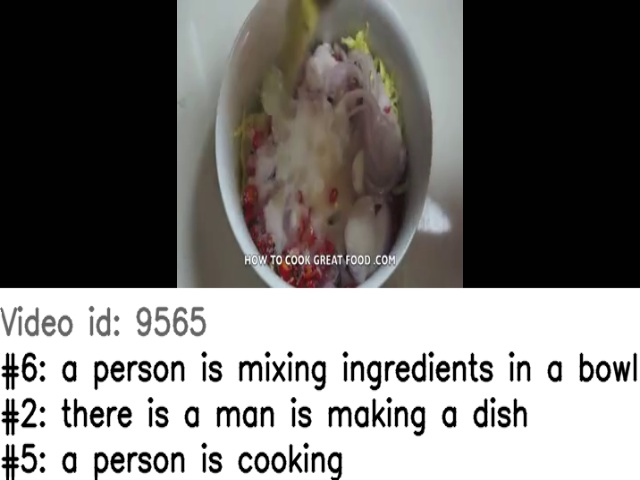
\includegraphics[width=0.30\linewidth]{images/9565.jpg}
    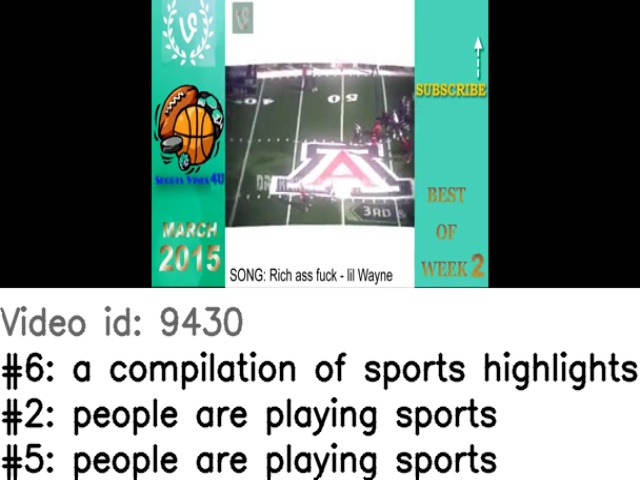
\includegraphics[width=0.30\linewidth]{images/9430.jpg}
    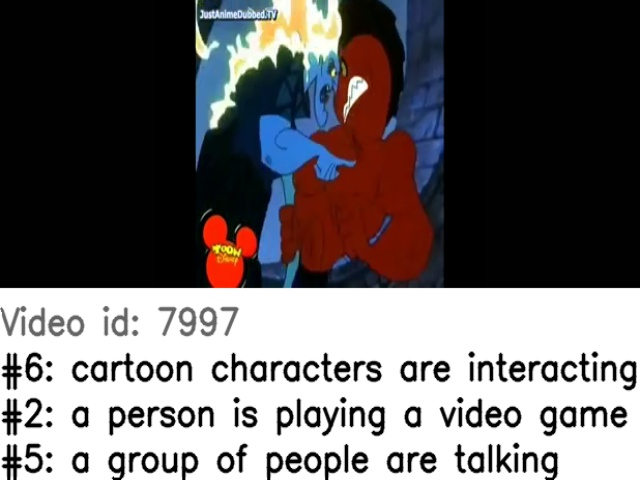
\includegraphics[width=0.30\linewidth]{images/7997.jpg}\\
    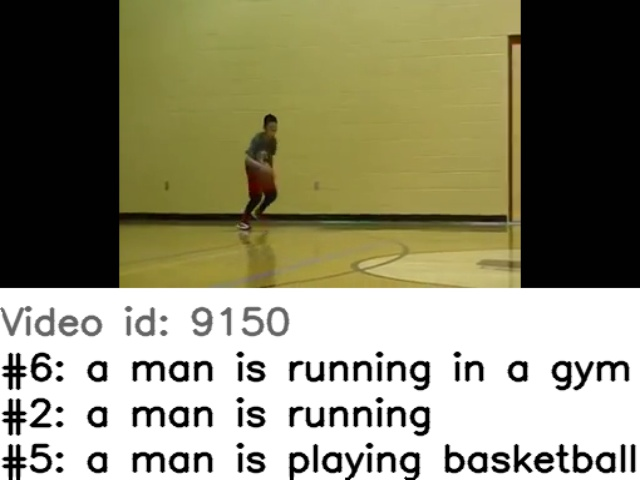
\includegraphics[width=0.30\linewidth]{images/9150.jpg}
    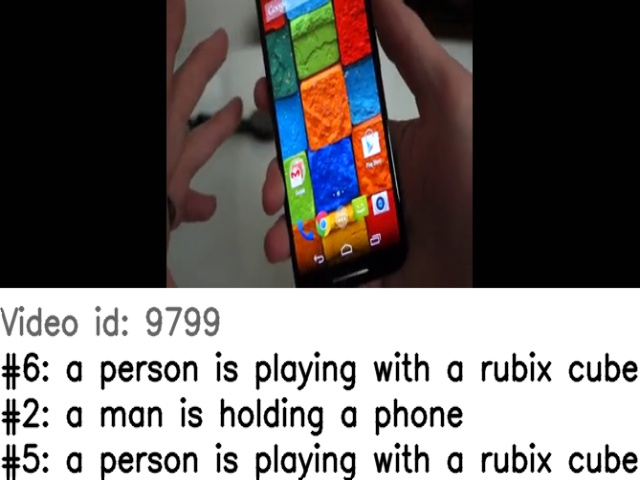
\includegraphics[width=0.30\linewidth]{images/9799.jpg}
    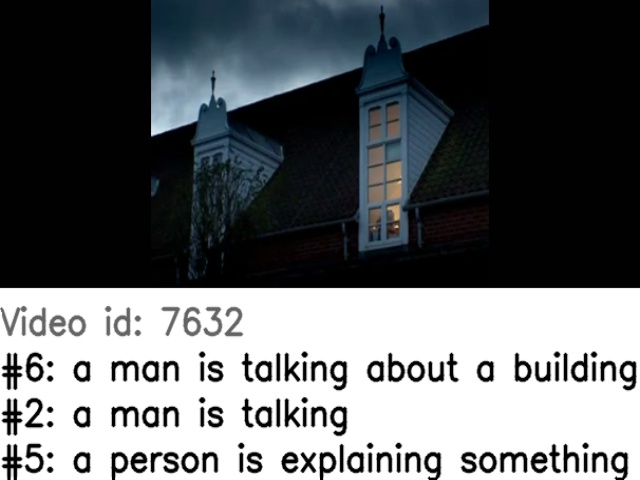
\includegraphics[width=0.30\linewidth]{images/7632.jpg}
  \end{center}
  \vspace*{-5mm}
  \caption{Sample captions generated for some test set videos. The
    first row shows samples where the evaluator model \#6 outperforms
    models \#2 and \#5, and the second row cases where the evaluator
    performs worse.}
  \label{fig:capSamps}
\end{figure*}

\begin{table*}[thp]
  \caption{Performance of various features and 
    network depths on the validation set of MSR-VTT}
  \newcommand{\modpar}[4]{%
    \multirow{2}{*}{\emph{#1}} & \multirow{2}{*}{#2} & \multirow{2}{*}{#3}
    & \multirow{2}{*}{#4}}
  \centering
  \newcommand{\bs}{\small\bf}
  \begin{tabular}{||c|c|c|c|c|c|c|c|c|}
    \hline\hline
    \bf\# &\bf init &\bf persist &\bf depth &\bf perplex &\bs BLEU-4 &\bs METEOR &\bs CIDEr &\bs ROUGE-L \\\hline\hline
    1 & dt  & gCNN+20Categ & 1  & 27.31 & 0.396 & 0.268 & 0.438 & 0.588 \\
    2 & dt  & gCNN+20Categ & 2  & 27.73 & 0.409 & 0.268 & 0.433 & 0.598 \\
    3 & dt  & gCNN+20Categ & 3  & 28.44 & 0.370 & 0.262 & 0.397 & 0.575 \\\hline
    4 & idt & gCNN+20Categ & 2  & 28.13 & 0.398 & 0.268 & 0.432 & 0.587 \\
    5 & dt  & c3dfc7       & 2  & 29.58 & 0.369 & 0.268 & 0.413 & 0.577 \\\hline
    6 & \multicolumn{4}{c|}{\em CNN evaluator based ensemble of best 4 models}
                                  & \bf0.411 & \bf0.277 & \bf0.464 & \bf0.596 \\\hline
    \hline
  \end{tabular}
  \label{tab:resultsVal}
\end{table*}

%% ---------------------------------------------------------------------------

\subsection{Challenge Results}

Since the CNN evaluator model performed the best on the validation set, we
submitted that result in the MSR-VTT Challenge.
%%
Our submission appears on the leaderboard as \emph{Aalto}.
%%
The submissions were evaluated on the blind test set using the above mentioned
four automatic metrics.
%%
These results are shown in Table~\ref{tab:resultsTestMet}.
%%
Our submission achieved the best scores in the CIDEr metric and was ranked
overall second considering the average ranking across the metrics.

The submissions were also subject to human evaluation as the automatic metrics
are known to deviate from human judgements.
%%
This was seen in previous captioning challenges in the case of both
image~\cite{CocoChallengeSlides} and
video~\cite{DBLP:journals/corr/RohrbachTRTPLCS16} data.
%%
The human evaluation was based on three criteria: Coherence (C1), Relevance (C2)
and Helpfulness for the blind (C3).
%%
Table~\ref{tab:resultsTestMet} presents the results of the evaluation.
%%
The overall ranking was obtained again by considering the mean ranking across
the three metrics.
%%
As per human judgement, our submission was ranked the first among the 22 entries
in the challenge.

Analyzing the two leaderboards, the automatic metric based one and the human
evaluation based one, we see that the disagreement between the two is relatively
minor, with most teams in the top 10 changing their ranking by only one
position.
%%
This can most likely be attributed to having a large number of 20 reference
captions per video for the evaluation.

\begin{table}[th]
  \caption{Top 5 teams as per metrics on the test set}
  \centering
  \newcommand{\bs}{\small\bf}
  \scalebox{0.9}{
  \begin{tabular}{||c|c|c|c|c|}
    \hline\hline
    \bf Team  &\bs BLEU-4 &\bs METEOR &\bs CIDEr &\bs ROUGE-L \\\hline\hline
    v2t\_navigator &\bf0.408 &\bf0.282 & 0.448 &\bf0.609 \\
    \bf Aalto      & 0.398 & 0.269 &0.457 & 0.598 \\
    VideoLAB       & 0.391 & 0.277 & 0.441 & 0.606 \\
    ruc-uva        & 0.387 & 0.269 &\bf0.459 & 0.587 \\
    Fudan-ILC      & 0.387 & 0.268 & 0.419 & 0.595 \\\hline
    \hline
  \end{tabular}}
  \label{tab:resultsTestMet}
\end{table}

\begin{table}[th]
        \caption{Top 5 teams as per human evaluation}
  \centering
  \newcommand{\bs}{\small\bf}
  \begin{tabular}{||c|c|c|c|}
    \hline\hline
    \bf Team  &\bs C1 &\bs C2 &\bs C3 \\\hline\hline
    \bf Aalto      & \bf3.263 & 3.104 & \bf3.244\\
    v2t\_navigator & 3.261 & 3.091 & 3.154 \\
    VideoLAB       & 3.237 & \bf3.109 & 3.143 \\
    Fudan-ILC      & 3.185 & 2.999 & 2.979 \\
    ruc-uva        & 3.225 & 2.997 & 2.933 \\\hline
    \hline
  \end{tabular}
  \label{tab:resultsTestHum}
\end{table}

%% ===========================================================================

\section{Conclusions}


\section{Summary of Results}
\fixme{About 2 pages, Fresh writing }
Summarizing results of both image and video, how they are similar and different
(for eg. kinds of mistakes made in video vs image).
